% !TEX program = xelatex
\documentclass[11pt,a4paper]{article}
\usepackage{kotex}
\setmainhangulfont{Malgun Gothic}
\setsanshangulfont{Malgun Gothic}
\usepackage{fontspec}
\setmainfont{TeX Gyre Pagella}
\setsansfont{TeX Gyre Heros}
\usepackage{amsmath,amssymb,mathtools,bm}
\usepackage{booktabs,longtable,tabularx,array}
\usepackage{geometry}
\geometry{top=2.05cm,bottom=2.15cm,left=2.05cm,right=2.05cm}
\usepackage{graphicx}
\graphicspath{{figures/}}
\usepackage{caption}
\captionsetup{font=small,labelfont=bf,labelsep=period}
\usepackage{enumitem}
\usepackage{xcolor}
\usepackage{fancyhdr}
\usepackage{float}
\usepackage[hidelinks]{hyperref}
\definecolor{navy}{HTML}{183B56}
\definecolor{teal}{HTML}{207F79}
\definecolor{amber}{HTML}{A96500}
\definecolor{crimson}{HTML}{A12B3B}
\definecolor{lightamber}{HTML}{FFF4DF}
\definecolor{lightblue}{HTML}{EAF2F6}
\definecolor{lightgray}{HTML}{F3F5F6}
\hypersetup{
  pdftitle={열원자 증기 FWM 스퀴징의 원치 않는 모드와 초과잡음},
  pdfauthor={GABES literature and model audit},
  pdfsubject={Balanced SQL, EOM sidebands, laser noise, hot-vapor Langevin noise},
  colorlinks=true,
  linkcolor=navy,
  citecolor=teal,
  urlcolor=navy
}
\pagestyle{fancy}
\fancyhf{}
\lhead{\small 열원자 FWM 초과잡음 조사}
\rhead{\small GABES 문헌ㆍ모델 감사}
\cfoot{\thepage}
\setlength{\headheight}{14pt}
\newcommand{\dd}{\mathrm d}
\newcommand{\ii}{\mathrm i}
\newcommand{\e}{\mathrm e}
\newcommand{\Tr}{\operatorname{Tr}}
\newcommand{\Rea}{\operatorname{Re}}
\newcommand{\Var}{\operatorname{Var}}
\newcommand{\Cov}{\operatorname{Cov}}
\newcommand{\MHz}{\,\mathrm{MHz}}
\newcommand{\kHz}{\,\mathrm{kHz}}
\newcommand{\GHz}{\,\mathrm{GHz}}
\newcommand{\dB}{\,\mathrm{dB}}
\newcommand{\degC}{\,^{\circ}\mathrm C}
\newcommand{\SQL}{\mathrm{SQL}}
\newcommand{\Rmix}{R_{\mathrm{mix}}}
\newcommand{\status}[1]{\textsc{#1}}
\newcommand{\established}{\textcolor{teal}{\status{established}}}
\newcommand{\inferred}{\textcolor{amber}{\status{inferred}}}
\newcommand{\openclaim}{\textcolor{crimson}{\status{open}}}
\newcommand{\ket}[1]{\lvert #1\rangle}
\newcommand{\enquote}[1]{“#1”}
\newcolumntype{Y}{>{\raggedright\arraybackslash}X}
\newcolumntype{L}[1]{>{\raggedright\arraybackslash}p{#1}}
\newcolumntype{C}[1]{>{\centering\arraybackslash}p{#1}}
\setlist[itemize]{leftmargin=1.45em,itemsep=2pt,topsep=4pt}
\setlist[enumerate]{leftmargin=1.65em,itemsep=3pt,topsep=4pt}
\sloppy
\title{\textbf{열원자 증기 Four-Wave Mixing 스퀴징에서\\
원치 않는 모드, EOM sideband, 레이저 및 원자 초과잡음}\\[7pt]
\large Balanced SQL 정규화와 GABES 기반 이론ㆍ수치 감사}
\author{GABES literature and model audit}
\date{2026년 8월 25일}
\begin{document}
\maketitle
\noindent
\fcolorbox{amber}{lightamber}{%
\begin{minipage}{0.945\textwidth}
\textbf{가장 중요한 결론.}
이상적인 독립 coherent sideband가 수동적으로 섞이는 것만으로는,
동일한 총 검출 파워와 동일한 전자 전달함수로 다시 측정한 SQL을 넘을 수 없다.
그 혼입은 스퀴징을 $0\dB$ 쪽으로 희석할 뿐이다.
따라서 Sim--Kim--Moon의 정확히 $50\%$ residual-carrier 조건에서 보이는
plotted-SQL-above 스펙트럼은 \enquote{carrier가 펌프에서 유래한 coherent light}라는
사실만으로 설명되지 않는다. 원자 매질에서의 비선형 잡음 전달, 레이저/EOM RF 잡음,
주파수별 balanced-detector 불일치, 포화ㆍintermodulation, 또는 SQL 기준의 조건
불일치 중 적어도 하나가 추가되어야 한다. 엄밀한 동일조건 SQL 초과 여부는 아직
열린 측정 문제다.
\end{minipage}}
\begin{abstract}
본 보고서는 열원자 $^{85}$Rb/$^{87}$Rb double-$\Lambda$ four-wave mixing(FWM)
intensity-difference squeezing에서 원치 않는 광학 모드가 loss보다 크게 성능을
악화시키고 논문에 그려진 SQL 기준선 위로 나타나는 관측을 조사한다. 먼저 multimode
coherent state의 Poisson/Skellam 통계와 동일조건 SQL을 이용해, 독립 coherent 혼입과
양 arm에 대칭이고 공분산에 정합된 post-loss는 정규화 잡음을 SQL 아래에서 SQL로만
이동시킨다는 정리를 보인다. 반대로 비대칭 loss나 고정된 subtraction weight,
super-Poissonian contaminant, 원자 매질의 Langevin diffusion, phase-to-amplitude
conversion, parasitic FWM/two-beam coupling, detector transfer mismatch, 또는 잘못된
SQL reference는 SQL 초과를 만들 수 있다.

Sim, Kim, Moon의 2025년 논문을 재검토한 결과, residual carrier/원하는 seed 비율은
$\ll0.5\%$, $0.5\%$, $12.5\%$, $25\%$, $50\%$이고 \enquote{$50\%$ 초과} 조건은 없다.
정확히 $50\%$ 곡선이 대부분의 분석 대역에서 논문에 그려진 SQL 기준선 위에 놓이지만,
각 조건에서 같은 총 검출 power로 SQL을 다시 측정했는지는 제시되지 않았고 power-slope
분석에도 이 조건이 포함되지 않는다. $12.5\%$와 $25\%$ slope ratio에 cell 전 입력비를
검출 shot-weight 비율인 것처럼 대입하면 $C_{\rm proxy}=4.229$, $4.284$를 얻지만,
증폭ㆍ흡수 뒤의 mode별 power가 없으므로 이 값은 비보정 empirical coefficient일 뿐
excess-noise transfer나 contaminant의 Fano factor를 정량적으로 지지하지 않는다.

Sim Fig.~3(a)의 같은 spectrum에는 $40$--$500\kHz$의 직접 $-7.8\dB$ IDS와
약 $2\MHz$의 좁은 noise peak가 함께 나타난다\cite{Sim2025}. 2023--2024년 내부
랩미팅 자료와 2026년 실험 로그에서도 대략 $1.5$--$2.4\MHz$의 feature가 반복되므로,
이를 현 setup의 국소적인 technical-noise 문제로 분류한다. 이 feature는 해당 주파수와
usable bandwidth를 훼손하지만, 저주파 $-7.8\dB$와의 공존은 broadband excess-noise
floor의 주원인일 필요가 없음을 시사한다. 정확한 전달 경로는 아직 열려 있다.

GABES/SABES 내부 코드를 사용해 온도별 증기 밀도와 감쇠 스케일, EOM/etalon 전력
순도, $121\degC$와 $0.32^\circ$에서 2차원 Maxwell 평균한 weak response를 재계산했다.
$795\,\mathrm{nm}$, $394.15\,\mathrm K$의 Planck 점유수는
$1.14\times10^{-20}$이다. 비공선 Raman Doppler rms는 $1.380\MHz$, Rb--Rb ground
collision 항은 $2.882\kHz$, 입력 transit floor는 $100\kHz$, 추가 optical-coherence
self-width는 $0.742\MHz$이다. 이들은 현재 코드 계수에 따른 결정론적 감쇠ㆍ응답
스케일이며 검증된 rate나 noise power가 아니다. 현재 GABES에는 microscopic
$D(\Omega)$가 없어 물리적 $S_-(\Omega)$를
예측하지 않는다.
\end{abstract}
\tableofcontents
\clearpage
%======================================================================
\section{조사의 범위와 판정 체계}
%======================================================================

본 조사의 질문은 세 문장으로 압축된다.
\begin{enumerate}
\item 이상적인 coherent light가 FWM twin beam에 독립적으로 섞일 때 왜 원칙적으로
SQL을 넘지 않는가?
\item 그런데 Sim--Kim--Moon 실험의 residual EOM carrier 조건에서는 왜 논문에 그린
SQL reference 위의 noise trace가 나타나는가?
\item hot vapor에서 \enquote{thermal noise}라고 부를 수 있는 실제 물리적 기작은
무엇이며, 현재 GABES가 그중 어디까지 계산하는가?
\end{enumerate}

결론의 강도를 혼동하지 않기 위해 표~\ref{tab:evidence-classes}의 네 층을 사용한다.
코드에서 숫자가 출력되었다는 사실은 자동으로 물리적 예측을 뜻하지 않는다.
\begin{table}[H]
\centering
\caption{본 보고서의 증거 등급.}
\label{tab:evidence-classes}
\begin{tabularx}{\textwidth}{L{2.7cm}Y L{3.1cm}}
\toprule
등급 & 의미 & 허용되는 문장\\
\midrule
\established & 명시된 가정 아래의 통계ㆍ공분산 정리, 또는 논문에 직접 보고된 측정 &
\enquote{반드시}, \enquote{측정되었다}\\
GABES/SABES 계산 & 저장소의 현재 결정론적 코드가 재현한 응답, 감쇠율 또는 광파워 &
\enquote{현재 모델에서 계산된다}\\
\inferred & 단순화된 sensitivity model이나 유효 파라미터로부터 얻은 해석 &
\enquote{시사한다}, \enquote{일관된다}\\
\openclaim & microscopic diffusion, 검출 전달함수 또는 같은 조건의 SQL trace가 없어
결정할 수 없는 물리적 귀속 & \enquote{추가 측정이 필요하다}\\
\bottomrule
\end{tabularx}
\end{table}

기준 실험 PDF는 \path{references/} 폴더에 있는 Sim--Kim--Moon의
single-diode-laser/EOM FWM squeezing 논문이고,
양자 fluctuation 전개의 기준 문서는
\path{docs/FWM physics and analytic reconstruction/} 아래의
\texttt{squeezing\_analytic\_reconstruction\_v2.tex}이다.

%======================================================================
\section{SQL, balanced detection, coherent 혼입의 정확한 정리}
%======================================================================

\subsection{동일조건 SQL과 Poisson/Skellam 통계}

검출창 하나에서 probe와 conjugate의 photocount를 $N_p,N_c$, 전기적 차감 가중치를
$w$라 하자. 서로 독립인 coherent state이면
\begin{equation}
N_p\sim\operatorname{Pois}(\mu_p),\qquad
N_c\sim\operatorname{Pois}(\mu_c),
\end{equation}
이고 $w=1$일 때 차이는 Skellam 분포를 따른다. 일반 $w$에서도
\begin{equation}
\langle D_w\rangle=\mu_p-w\mu_c,\qquad
\Var(D_w)=\mu_p+w^2\mu_c,\quad D_w=N_p-wN_c.
\label{eq:coherent-sql}
\end{equation}
따라서 이 측정의 coherent-state SQL은
\begin{equation}
V_{\SQL,w}=\mu_p+w^2\mu_c.
\label{eq:same-condition-sql}
\end{equation}
여기서 중요한 말은 \enquote{동일조건}이다. 비교 SQL은 실제 측정과 동일한 검출
파워, $w$, photodiode responsivity, $H_p(\Omega),H_c(\Omega)$, RBW/VBW 및
dark-noise 처리를 가져야 한다.

서로 다른 주파수나 공간 모드의 coherent 성분이 photodiode에서 서로 직교하고
검출 대역 내 beat를 만들지 않는다면, 총 count는 독립 Poisson 변수의 합이므로
여전히 Poisson이다. 그러나 광원이 다르다는 사실 자체가 shot-noise limited임을
보장하지 않는다. 각 광원에 classical RIN이나 phase noise가 있으면 Poisson 평균
자체가 시간에 따라 흔들리고, 그 결과는 compound Poisson 또는 super-Poissonian
통계가 된다.

\subsection{독립 coherent contaminant는 SQL을 넘지 못한다}

원래 twin beam의 같은 조건 shot-noise weight를 $S$, 정규화 difference noise를
$R_0\le1$, 독립 contaminant의 shot-noise weight를 $U$, 그 Fano-like excess factor를
$F_U$라 두면
\begin{equation}
\Rmix=\frac{R_0S+F_UU}{S+U}
=\frac{R_0+F_Ur}{1+r},\qquad r\equiv U/S.
\label{eq:mixing-general}
\end{equation}
이상적인 coherent contaminant에는 $F_U=1$이므로
\begin{equation}
\boxed{\Rmix=\frac{R_0+r}{1+r}
=1-\frac{1-R_0}{1+r}\le1.}
\label{eq:coherent-bound}
\end{equation}
한쪽 photodiode에만 혼입되어도 그 파워를 SQL 분모에 동일하게 포함하면 결론은 같다.
SQL 초과 조건은
\begin{equation}
\boxed{\Rmix>1\quad\Longleftrightarrow\quad
r(F_U-1)>1-R_0,}
\qquad
F_U>1+\frac{1-R_0}{r}.
\label{eq:fano-threshold}
\end{equation}
따라서 super-SQL 관측은 이상적인 coherent admixture 가정 중 적어도 하나가
깨졌다는 진단이다.

\begin{figure}[H]
\centering
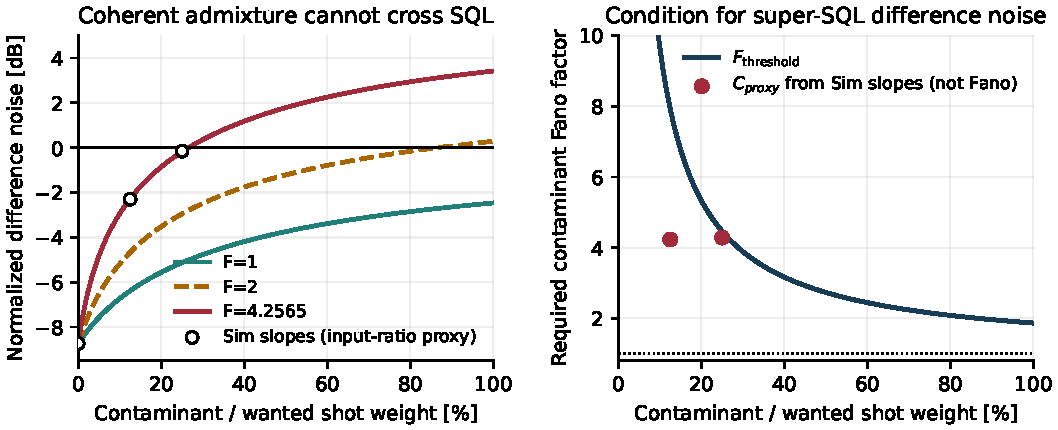
\includegraphics[width=\textwidth]{noise_mixing.pdf}
\caption{Sim 논문의 $R_0=0.134$ slope ratio를 시작점으로 한 혼입 sensitivity.
$F=1$ coherent 곡선은 모든 검출 shot-weight 혼입비에서 SQL 아래에 남는다.
붉은 $4.2565$ 곡선과 점은 cell 전 입력 carrier/seed 비율을 검출 shot-weight로
대입한 비보정 $C_{\rm proxy}$의 시각화일 뿐, Fano factor나 transfer 측정값이 아니다.}
\label{fig:noise-mixing}
\end{figure}

\subsection{대칭ㆍ정합 post-loss는 SQL을 넘지 못한다}

두 arm이 같은 transmissivity $\eta$를 갖고 subtraction weight가 공분산에 정합되어
있다면, 스퀴즈된 mode가 passive loss를 지나 vacuum과 섞일 때
\begin{equation}
R_{\rm loss}=\eta R_0+(1-\eta).
\label{eq:pure-loss}
\end{equation}
$0\le R_0\le1$이면 $R_{\rm loss}\le1$이다. 그러나 일반적인 arm별 효율
$\eta_p,\eta_c$와 고정 weight $w$에서는, $V_{ij}=\Cov(N_i,N_j)$와
$\mu_i=\langle N_i\rangle$로 두면
\begin{align}
V'_-={}&\eta_p^2V_{pp}+w^2\eta_c^2V_{cc}-2w\eta_p\eta_cV_{pc}\nonumber\\
&+\eta_p(1-\eta_p)\mu_p+w^2\eta_c(1-\eta_c)\mu_c,\\
S'_{\rm SQL}={}&\eta_p\mu_p+w^2\eta_c\mu_c,
\label{eq:unequal-loss}
\end{align}
이므로 $\eta_p\ne\eta_c$ 또는 잘못된 $w$는 각 arm의 큰 thermal marginal을 드러내
$V'_-/S'_{\rm SQL}>1$을 만들 수 있다. 즉
\enquote{모든 pure loss가 SQL을 넘지 못한다}는 명제는 성립하지 않는다
\cite{Jasperse2011}. 셀 내부 distributed absorption도 단순 대칭 post-loss가 아니다.
Jasperse et al.은 이를 위치별 beam-splitter vacuum 주입으로 다루며, 별도의
spontaneous-emission/fluorescence reservoir는 microscopic Langevin channel로
분리해야 한다\cite{Glorieux2010,Slusher1987,Hsu2006}.

\subsection{EOM이 coherent input에 하는 일과 하지 않는 일}

이상적인 phase modulator의 unitary는 coherent carrier를
\begin{equation}
\ket{\alpha}_{0}\longrightarrow
\bigotimes_{n=-\infty}^{\infty}
\ket{\alpha J_n(\beta)\e^{\ii n\phi}}_{\omega_0+n\Omega_m}
\end{equation}
로 보낸다. 각 sideband는 coherent이고 결정론적 modulation 자체는 초과잡음을
만들지 않는다. 실제 장치에서는 $\beta(t)$와 $\phi(t)$가 RF source의 AM/PM noise를
가지며, ECDL carrier의 주파수ㆍ위상 잡음도 모든 sideband에 상관된 형태로 복제된다.
원자 매질이 이를 서로 다른 complex susceptibility로 처리하면 common-mode였던
noise가 difference amplitude noise로 변환될 수 있다.

Photodiode 전류에는
\begin{equation}
I(t)\supset 2\Rea\!\left[
\alpha_m\alpha_n^*\e^{-\ii(\omega_m-\omega_n)t}\right]
\label{eq:beat}
\end{equation}
가 존재한다. $|\omega_m-\omega_n|$가 선형 detector/ESA 대역 밖이면 평균되어
사라지고, GHz beat의 phase-noise가 스스로 MHz baseband로 이동하지는 않는다. 가까운
line pair가 실제 검출 대역에 있거나, 원자 매질의 PM-to-AM 변환, detector/TIA의
비선형 mixingㆍintermodulation, aliasing 또는 RF pickup이 명시적으로 있을 때에만
\enquote{서로 다른 주파수라서 무관하다}는 단순화가 실패한다.

\subsection{balanced detection이 실제로 상쇄하는 것}

일반적인 차동 PSD는
\begin{align}
S_-(\Omega)={}&|w_pH_p|^2S_{pp}+|w_cH_c|^2S_{cc}\nonumber\\
&-2\Rea\!\left[w_pw_c^*H_pH_c^*S_{pc}\right]+S_{\rm el}.
\label{eq:balanced-psd}
\end{align}
공통 excess noise는 $S_{pc}$가 충분히 크고 두 전달함수와 delay가 맞을 때만 상쇄된다.
Yuen--Chan의 이론(및 heterodyne vacuum-sideband 항을 바로잡은 erratum)과
Abbas--Chan--Yee의 실험은 50:50 beam splitter 두 출력을
coherent subtraction하여 같은 LO의 excess noise를 억제할 수 있음을 보였다
\cite{YuenChan1983,YuenChan1983Erratum,Abbas1983}. 후자의 서로 다른 광주파수는 같은 레이저에서 AOM으로
$80\MHz$ 이동한 것이며, 독립 레이저 두 대의 임의 잡음이 자동으로 사라진다는
실험은 아니다. Differential delay $\tau$가 있으면 공통 noise의 잔류가
$2S(f)[1-\cos(2\pi f\tau)]$처럼 주파수에 따라 증가할 수 있다\cite{Abbas1983}.

%======================================================================
\section{참조 논문들의 정확한 의미와 Sim 데이터 재해석}
%======================================================================

\subsection{SQL/balanced-detection 로컬 문헌이 지지하는 범위}

\begin{table}[H]
\centering
\caption{사용자가 제공한 SQL 관련 문헌의 직접 증거와 과잉 일반화 방지.}
\label{tab:sql-literature}
\small
\begin{tabularx}{\textwidth}{L{3.0cm}Y Y}
\toprule
문헌 & 직접 지지하는 내용 & 지지하지 않는 내용\\
\midrule
Yuen--Chan 및 erratum\cite{YuenChan1983,YuenChan1983Erratum} & homodyne/heterodyne의 LO excess-noise 항과
double-detector coherent subtraction & 임의의 독립 source가 모두 SQL이라는 실험\\
Abbas--Chan--Yee\cite{Abbas1983} & 같은 laser에서 AOM으로 $80\MHz$ 이동한 signal과
LO에서 약 $14\dB$ excess-noise 억제 & 서로 독립인 두 레이저의 무조건적 상쇄\\
Painchaud et al.\cite{Painchaud2009} & coherent receiver의 splitting imbalance,
CMRR, differential delay와 주파수별 rejection & shot-noise spectrum을 측정한 SQL 검증\\
Brumfield--Wysocki\cite{Brumfield2012} & CMRR로 RIN을 억제하고 shot noise가 비상관
합으로 남는 near-shot-noise detector budget & 서로 다른 주파수ㆍsource의 보편 정리\\
Lvovsky--Raymer\cite{LvovskyRaymer2009} & balanced homodyne의 mode selectivity,
efficiency를 vacuum loss로 표현, electronic-noise clearance & direct twin-beam에서
모든 unwanted mode가 단순 loss라는 주장\\
\bottomrule
\end{tabularx}
\end{table}

\subsection{Sim--Kim--Moon 논문의 실제 관측}

Sim, Kim, Moon은 single-diode-laser/EOM seed 방식으로 $^{85}$Rb에서 직접
$-7.8\dB$, IDS/SQL power-slope ratio로 $-8.7\dB$를 보고했고, 약
$3.5\MHz$의 squeezing 대역을 제시했다\cite{Sim2025}. 논문이 말하는 SQL은 cell 앞의
pump를 50:50으로 나눈 coherent beam pair의 difference noise다. Fig.~3(a)의 동일
spectrum에서 $40$--$500\kHz$의 최대 squeezing과 약 $2\MHz$의 좁은 peak가 함께
보이며, 저자들은 후자를 laser-source electronic noise에 귀속한다.

Sim 본문이 정의한 residual carrier/원하는 probe seed input power ratio는 정확히
\[
\ll0.5\%,\quad0.5\%,\quad12.5\%,\quad25\%,\quad50\%
\]
이다. 다만 Fig.~5(a,b)와 Fig.~6 caption은 같은 비를
\enquote{probe-seed to carrier/multimode ratio}로 반대로 적어 원문 내부 정의가
일치하지 않는다. 본 보고서는 본문 정의를 따라 위 순서로 표기하지만, 이 불일치와
post-cell mode별 power 부재 때문에 그 비를 검출 shot-weight로 확정하지 않는다.
Fig.~5(b)의 정확히 $50\%$ 곡선은 $0$--$4\MHz$ 대부분에서 논문에 그려진 SQL
reference 위에 있다. 그러나 각 혼입 조건에서 동일 총 검출 power와 전달함수로 SQL을
재측정했다는 절차가 없고 Fig.~6의 power-slope 분석도 $\ll0.5\%$, $12.5\%$, $25\%$만
포함한다. 따라서 엄밀한 동일조건 super-SQL 여부는
\openclaim 이며, 직접 증거는 \enquote{$50\%$ spectrum이 plotted SQL reference 위에
나타난다}까지다.

\begin{table}[H]
\centering
\caption{Sim Fig.~6 slope ratio와 입력비를 대입한 비보정 proxy 역산.}
\label{tab:sim-fano}
\begin{tabular}{C{3.4cm}C{2.8cm}C{2.8cm}L{5.0cm}}
\toprule
입력 carrier/seed ratio & 측정 $R$ & $10\log_{10}R$ & 비보정 $C_{\rm proxy}$\\
\midrule
$\ll0.5\%$ & 0.134 & $-8.73\dB$ & 기준점\\
$12.5\%$ & 0.589 & $-2.30\dB$ & 4.229\\
$25\%$ & 0.964 & $-0.16\dB$ & 4.284\\
\bottomrule
\end{tabular}
\end{table}

표~\ref{tab:sim-fano}의 단순 대입은
\begin{equation}
C_{\rm proxy}=\frac{R_{\rm obs}(1+r_{\rm in})-R_0}{r_{\rm in}}
\label{eq:effective-fano}
\end{equation}
을 썼다. 여기서 $r_{\rm in}$은 cell 전 입력비인 반면, 식~\eqref{eq:mixing-general}의
$r=U/S$는 post-cell detected shot-noise weight 비여야 한다. 원하는 seed는 FWM에서
증폭되고 carrier는 서로 다른 absorption, gain, spatial overlap을 겪으므로 두 비는
일반적으로 같지 않다. 따라서 $4.229$와 $4.284$가 가깝다는 사실은 입력비에 대한
empirical slope가 비슷하다는 것만 말하며, 추가 noise transfer나 carrier의 Fano
factor를 정량적으로 입증하지 않는다. 이 값은 필요한 post-cell power ledger를 얻기
전까지 illustration으로만 보존한다.

논문에 인쇄된 \enquote{$0.5\%$ carrier가 squeezing bandwidth를 $0.8\GHz$
감소시킨다}는 문구는 Fig.~5의 MHz 축과 전체 $3.5\MHz$ 대역보다 두 자릿수 이상
크므로 단위 오기 가능성이 높다. 본 보고서는 이를 $0.8\MHz$라는 확정값으로 고치지
않고, 원문 내부 불일치로 기록한다.

\subsection{gain/loss sanity check가 말해 주는 것}
\label{sec:gain-loss-sanity}

이상적인 seeded parametric amplifier에서
\begin{equation}
R_{\rm ideal}=\frac{1}{2G-1}.
\end{equation}
$G\simeq15$이면 $R_{\rm ideal}=1/29\simeq-14.6\dB$이고, 논문이 인용한 총 loss
$13.5\%$를 단순 symmetric post-loss로 넣으면
\begin{equation}
R_{\rm det}=0.135+0.865/29\simeq0.165\simeq-7.8\dB.
\end{equation}
이는 직접 측정 $-7.8\dB$와 가깝다. 그러나 같은 계산에서 $G$와 $\eta$를 이상적
Bogoliubov map에 넣었기 때문에 가능한 algebraic consistency check일 뿐이다.
원자 매질의 distributed absorption과 diffusion을 검증하거나, 현재 GABES의 큰
mean-field gain을 물리적 squeezing으로 바꾸는 근거는 아니다.

\subsection{현 셋업에서 반복되는 1.8--2 MHz noise feature}
\label{sec:setup-2mhz}

Sim 논문의 Fig.~3(a)는 $40$--$500\kHz$에서 직접 $-7.8\dB$ IDS와 약
$3.5\MHz$의 squeezing bandwidth를 보고하는 동시에, 약 $2\MHz$의 좁은 peak를
laser-source electronic noise에 귀속한다\cite{Sim2025}. 따라서 이 feature가 있는
동일 spectrum에서도 저주파 squeezing은 절~\ref{sec:gain-loss-sanity}의
loss-only sanity check가 주는
$-7.8\dB$에 도달한다. 이는 측정된 공존 관계다. 이로부터 narrow peak가 해당 대역과
usable bandwidth를 훼손하되 저주파ㆍbroadband excess-noise floor의 주원인일 필요는
없다고 추정할 수 있지만, 후자는 인과 측정이 아니다.

내부 자료는 이 feature가 일회성 artifact가 아니라 동일 setup 계보에서 반복되었음을
보인다. 230630 자료의 slides~34--36은 EOM/seed-path noise가 FWM difference signal로
전달됨을, 230728 자료의 slides~5와 22는 EOM 통과 뒤 noise 증가와 residual-carrier
의존성을 기록한다\cite{SimLab230630,SimLab230728}. 231020 slide~15에서는 사용하지
않던 laser와 driver를 제거한 뒤 $1.8$--$2\MHz$ 부근의 넓은 구조가 감소했고,
231110 자료는 electrical noise가 squeezing signal에 그대로 들어오는 관측과
$100\kHz$--$4\MHz$ passive-filter 설계를 제시한다
\cite{SimLab231020,SimLab231110}. 231208 slide~8은 $1\MHz$ 및 $1.5$--$2\MHz$의
noise를 명시하고, 231222 slides~8--11은 spectrum analyser 자체보다
laser/PZT/MOPA 계통을 의심하며 여러 inductor를 비교한다
\cite{SimLab231208,SimLab231222}. 240213 자료에서는 $100\kHz$에서
$6.9\pm0.2\dB$를 관측한 setup의 frequency trace에 near-$2\MHz$ narrow feature가
남아 있고, 완만한 고주파 roll-off의 별도 후보로 slow-light와 PD RF imbalance를
제시한다\cite{SimLab240213}.

2026-05-28 로그에는 약 $2.4\MHz$ peak와 noise eater 재도입 필요성이 기록되지만,
그날은 upstream alignment 문제로 squeezing을 측정하지 못했다
\cite{ExperimentLog20260528}. 2026-07-13 로그는 현 setup에서 약 $1.3\MHz$부터
FWM noise가 상승하고 약 $2\MHz$의 큰 narrow peak와 pedestal이 나타나 usable
bandwidth를 제한한다고 기록한다\cite{ExperimentLog20260713}. 서로 다른 시기의
중심주파수가 대략 $1.5$--$2.4\MHz$에 걸치고, laser/driver 분리와 passive/etalon
filtering에서 크기가 변했다. Noise eater는 정렬 난도로 인해 검증이 끝나지 않았다.
따라서 고정된 보편적 공명보다 setup-specific technical feature로 다루는 편이 증거에
맞다. 안정적인 제거가 아직 되지 않았으므로 추가 분석은 필요하지만, 이 narrow
feature를 residual-carrier 조건의
broadband plotted-SQL-above noise나 원자 thermal excess noise와 동일시해서는 안 된다.

Palmer et al.의 $1.8\MHz$는 intracavity EOM을 이용한 특정 frequency lock의
feedback-loop resonance 및 closed-loop bandwidth 사례다\cite{Palmer2022}. 현재
feature의 원인을 직접 입증하지 않는다. Rb FWM의 주파수 의존 squeezingㆍcorrelation도
수 MHz보다 넓은 범위와 group-delay/transfer 의존성을 보이므로, $2\MHz$를 열원자
FWM의 보편적 atomic cutoff로 둘 근거는 없다\cite{McCormick2008,deAraujo2024}.

%======================================================================
\section{hot-vapor thermal/excess noise의 물리적 분류}
%======================================================================

\subsection{세 가지 서로 다른 thermal의 의미}

\begin{enumerate}
\item \textbf{두-mode squeezed state의 thermal marginal.} 각 arm만 보면 photon-number
분산이 thermal처럼 보일 수 있지만, 두 arm의 covariance가 difference에서 이를
상쇄한다. 이는 주위 온도의 blackbody photon bath와 다르다.
\item \textbf{열원자의 운동ㆍpopulationㆍcollision.} Maxwell velocity 분포,
transit, hyperfine population, collision, radiation trapping 등이 susceptibility와
reservoir diffusion을 바꾼다.
\item \textbf{generic technical excess noise.} ECDL/TA RIN과 frequency noise,
servo bump, EOM RF AM/PM noise, beam pointing, detector electronics는 thermal이
아니지만 실험 스펙트럼에서는 함께 excess noise로 보일 수 있다.
\end{enumerate}

$795\,\mathrm{nm}$와 $T=394.15\,\mathrm K$에서 Planck 점유수는
\begin{equation}
\bar n_{\rm BB}=\frac{1}{\exp(hc/\lambda k_BT)-1}
=1.14\times10^{-20}.
\end{equation}
따라서 cell 주변의 직접적인 optical blackbody photon은 후보에서 제외할 수 있다.
반면 $3.035\GHz$ ground hyperfine splitting에는
$h\nu/k_BT=3.70\times10^{-4}$이므로 비펌프 열평형에서는 두 manifold 사이의
Boltzmann suppression이 거의 없다. 실제 실험의 population은 degeneracy와 강한
optical pumping을 포함한 driven OBE가 결정하며, 이 사실은 detector에 optical
thermal bath가 들어온다는 뜻이 아니다.

\subsection{기작별 noise ledger}

\begin{longtable}{L{3.0cm}L{4.0cm}L{4.0cm}L{4.0cm}}
\caption{열원자 FWM에서 가능한 초과잡음 기작, 예상 signature와 판별법.}
\label{tab:mechanism-ledger}\\
\toprule
기작 & 물리적 경로 & 예상 의존성ㆍsignature & 우선 판별법\\
\midrule
\endfirsthead
\toprule
기작 & 물리적 경로 & 예상 의존성ㆍsignature & 우선 판별법\\
\midrule
\endhead
\midrule
\multicolumn{4}{r}{\small 다음 페이지에 계속}\\
\endfoot
\bottomrule
\endlastfoot

Distributed absorption & 셀의 각 위치에서 vacuum reservoir가 들어오고 뒤쪽 gain이
이를 증폭 & post-cell loss와 다른 온도ㆍdetuningㆍ길이 의존성
\cite{Jasperse2011,Turnbull2013} & pump-off transmission과 gain/absorption의
longitudinal model 비교\\

Spontaneous/Raman fluorescence & excited population과 Raman channel의 비상관 photon이
검출 mode에 유입 & 인접한 hot-vapor biphotonㆍdegenerate FWMㆍPSR 배치에서 확인된
후보이며 현재 bright seeded Rb double-$\Lambda$의 크기는 미결정
\cite{Shu2016,Wang2023,Hsu2006} & cell 측면 $90^\circ$
fluorescence와 forward mode를 동시 측정\\

Vacuum side-mode FWM & 입사광은 shot-noise limited여도 원자증기가 vacuum side modes를
증폭 & detuning별 excess spectrum; 원자 없는 bypass에서는 사라짐\cite{Davis1995}
& pump/temperature/detuning을 바꾼 single-beam transmission-noise spectroscopy\\

Parasitic FWM 및 two-beam coupling & unwanted carrier/seed와 pump가 atomic grating,
교차 gain, vacuum amplification을 형성 & 상대각, 겹침, seed power, phase에 민감;
원자 linewidth 규모 feature\cite{Wu2021} & carrier phaseㆍ각도ㆍimage planeㆍoverlap
스캔\\

Phase-to-amplitude conversion & laser frequency/phase noise가 dispersive atomic
slope에서 intensity noise로 변환 & detuning에 따라 correlation 부호와 peak가 바뀜
\cite{McIntyre1993,Martinelli2004,deAlmeida2025} & 독립 frequency-noise 측정과
$\partial T/\partial\Delta$를 이용한 transfer 비교\\

Doppler/velocity classes & 각 velocity class가 다른 one/two-photon detuning과 gain,
diffusion을 가짐 & angle과 $\sqrt{T}$에 따른 Raman Gaussian scale & crossing angle을
줄이고 velocity-class-resolved model과 비교\\

Rb--Rb collision 및 dephasing & coherence damping, velocity-changing collision,
population fluctuation & density에 따라 증가; 고온에서 gain 증가와 경쟁
\cite{Glorieux2023} & 온도와
cell length를 분리하고 linewidth/fluorescence를 동시 fit\\

Transit-time statistics & 원자가 유한 beam을 드나들며 coherence와 population을 reload &
waist에 따라 corner가 대략 $v_{\perp}/w$로 이동 & pump/probe waist를 독립 변경\\

Spin/population noise & 열평형 및 optical pumping population fluctuation이 susceptibility를
변조 & magnetic field, polarization, pump power에 민감\cite{Swar2018} & spin-noise,
polarization 및 magnetic-field scan\\

Radiation trapping/reabsorption & 방출 photon의 재흡수가 optical pumping과 coherence
decay를 변화 & density와 cell geometry에 강하게 의존, 긴 decay tail
\cite{Matsko2001,Rosenberry2007} & pump-off time decay와 cell geometry 비교\\

Spatial multimode mismatch & detector가 상관 mode 외 다른 squeezed/uncorrelated mode를
다른 비율로 모음 & aperture, imaging, homodyne visibility, alignment 의존;
단순 loss보다 빠른 악화 가능\cite{Gupta2020} & far-field/near-field aperture와
mode-resolved detection\\

Pump scatter & 강한 pump의 stray light가 한 detector에 유입 & pump power, iris,
polarization, cell window에 민감; 완전 흡수점에서 SQL 초과 가능
\cite{Jasperse2011} & pump-block, spatial filter와 scatter camera\\

Self-focusing/공간 재형성 & 비선형 굴절률과 multiwave mixing이 mode geometry와
검출 overlap을 바꿈 & detuning, pump power, polarization에 민감\cite{Ho1991} &
near/far-field beam profile과 aperture scan\\

Laser/EOM/TA technical noise & RIN, frequency noise, servo resonance, RF AM/PM noise가
원자 slope에서 비대칭 전달 & servo gain과 actuator 변경 시 peak 이동; bypass/hot-cell에
따라 크기 변화\cite{Sim2025,SimLab231020,SimLab231110,SimLab231208,
SimLab231222,SimLab240213,Wu2019,McIntyre1993,Martinelli2004,deAlmeida2025} &
RINㆍfrequency-noiseㆍRF phase noise를 동시에 측정; 내부 provenance는
절~\ref{sec:setup-2mhz}, Palmer는 별도 servo 사례\\

Detector mismatch/nonlinearity & $H_p\ne H_c$, delay, CMRR, TIA gain, saturation,
intermodulation & DC balance가 맞아도 RF에서 잔류; optical power에 비선형 & frequency별
CMRR/delay와 detector power sweep\cite{Painchaud2009,McKenzie2007}\\

SQL calibration mismatch & actual total power/weight/RBW/dark 처리와 reference가 다름 &
다른 조건으로 얻은 0-dB 선; power slope가 정확히 선형이 아님 & 같은 shot-noise-limited
beam과 동일 acquisition setting으로 즉시 교차측정\\
\end{longtable}

Hot-vapor FWM의 낮은 주파수 한계가 본질적인 원자 bandwidth만은 아니라는 직접 사례로,
dual seeding은 seed excess noise와 gain-fluctuation imbalance를 상쇄해
$10\,\mathrm{Hz}$ 아래까지 squeezing을 확장했다\cite{Wu2019}. 초기 원자 FWM과
인접한 PSR/hot-vapor 배치에서는
spontaneous emission, dephasing, fluorescence가 squeezing을 제한할 수 있다
\cite{Slusher1987,Hsu2006}. 다만 후자의 geometry와 nonlinear process는 Sim의 bright
seeded Rb double-$\Lambda$ FWM과 같지 않다. 이 문헌들은 후보 reservoir channel의
존재만 뒷받침하며, 현재 실험에서 collision/fluorescence의 크기나 우세성을 입증하지
않는다.

%======================================================================
\section{양자 Langevin 기반의 필요한 이론 구조}
%======================================================================

\subsection{pumped atomic state에서 fluctuation을 선형화하기}

평균 OBE는 원자 density operator의 기대값만 다룬다. 물리적 squeezing에는
Heisenberg--Langevin operator와 그 correlation이 필요하다. Pump가 만든 정상상태
$\bar{\bm\sigma}(\bm v)$ 주위에서 원자 fluctuation을 선형화하면 개략적으로
\begin{equation}
\partial_t\delta\hat{\bm\sigma}_{\bm v}
=A_{\bm v}\delta\hat{\bm\sigma}_{\bm v}
+G_{\bm v}\delta\hat{\bm a}
+\hat{\bm F}_{\bm v}.
\label{eq:atomic-langevin}
\end{equation}
$A_{\bm v}$는 pumped Liouvillian의 Jacobian이고, Doppler shift는 각 field에 대해
$\Delta_j\rightarrow\Delta_j-\bm k_j\!\cdot\!\bm v$로 들어간다. Reservoir는
\begin{align}
[\hat{\bm F}_{\bm v}(z,\Omega),
\hat{\bm F}_{\bm v'}^\dagger(z',\Omega')]&=
2\pi J_{F,\bm v}\delta_{\bm v\bm v'}\delta(z-z')\delta(\Omega-\Omega'),\\
\tfrac12\langle\{\hat{\bm F}_{\bm v},
\hat{\bm F}_{\bm v'}^\dagger\}\rangle&=
2\pi N_{\bm v}\delta_{\bm v\bm v'}\delta(z-z')\delta(\Omega-\Omega')
\end{align}
로 기술한다. $N_{\bm v}$ 또는 이에 상응하는 diffusion coefficient는 pumped Lindblad
collapse operators와 steady-state population으로부터 generalized Einstein relation을
통해 유도해야 한다. 감쇠율만 $A$에 추가하고 대응 diffusion을 생략하면 commutator와
output noise가 동시에 틀린다. Double-$\Lambda$ microscopic Langevin 접근은
Lukin et al.과 Glorieux et al.에 제시되어 있다\cite{Lukin1999,Glorieux2010}.
다만 Glorieux의 해당 모델은 cold-atom 근사로 Doppler와 transit을 제외하므로 여기서는
구조적 기준으로만 쓴다. Complex gain/loss와 nonlinear coupling에서 필요한 reservoir
noise의 macroscopic 구성은 Jiang--Mei--Du 및 erratum이 보완한다
\cite{Jiang2023,Jiang2025Erratum}; hot-vapor의 velocity-changing collision과 diffusion은
별도로 유도해야 한다.

\subsection{원자 제거 후 공간 전파와 commutator 조건}

원자 fluctuation을 frequency domain에서 제거하면 두-mode Nambu vector
\begin{equation}
\hat{\bm A}(z,\Omega)=
\begin{pmatrix}\delta\hat a_p(z,\Omega)\\
\delta\hat a_c^\dagger(z,-\Omega)\end{pmatrix},
\qquad J=\operatorname{diag}(1,-1)
\end{equation}
에 대해
\begin{equation}
\partial_z\hat{\bm A}=M_q(z,\Omega)\hat{\bm A}
+B(z,\Omega)\hat{\bm F}(z,\Omega)
\label{eq:spatial-langevin}
\end{equation}
를 얻는다. 형식해는
\begin{equation}
\hat{\bm A}_{\rm out}=T(L,0)\hat{\bm A}_{\rm in}
+\int_0^L T(L,z)B(z)\hat{\bm F}(z)\dd z.
\end{equation}
출력 commutator 보존은
\begin{equation}
TJT^\dagger+\int_0^LT(L,z)BJ_FB^\dagger T^\dagger(L,z)\dd z=J,
\label{eq:commutator-integral}
\end{equation}
또는 local하게
\begin{equation}
\boxed{M_qJ+JM_q^\dagger+BJ_FB^\dagger=0}
\label{eq:physical-realizability}
\end{equation}
을 요구한다. 이는 gain/loss가 필요한 reservoir port를 분류하지만 symmetrized
diffusion의 온도와 excess population을 정하지는 않는다. 따라서 commutator defect를
독립 vacuum port로 닫는 algebraic fixture는 코드 검증에는 유용해도 atomic-noise
prediction이 아니다. Phase-insensitive amplifier의 최소 added-noise 한계와도 가정
범위를 구분해야 한다\cite{Caves1982}.

\subsection{공분산 전파와 velocity-class 합산}

Symmetrized diffusion을 $D=BNB^\dagger$라 하면
\begin{equation}
\boxed{V_{\rm out}=TV_{\rm in}T^\dagger+W(L),\qquad
W(L)=\int_0^LT(L,z)D(z)T^\dagger(L,z)\dd z.}
\label{eq:covariance-propagation}
\end{equation}
$M_q,D$가 한 segment에서 상수이면
\begin{equation}
\frac{\dd W}{\dd L}=M_qW+WM_q^\dagger+D,\qquad W(0)=0,
\label{eq:lyapunov}
\end{equation}
이고 Van Loan block exponential로 안정적으로 계산할 수 있다. 종방향 pump depletion,
density gradient, Gaussian overlap이 있으면 segment마다
\begin{equation}
V_{k+1}=T_kV_kT_k^\dagger+W_k
\end{equation}
를 합성한다. Collisionless 또는 fixed-velocity 근사에서만 서로 독립인 velocity
class를 noise power/covariance로 더할 수 있고, velocity-averaged Langevin amplitude를
만든 뒤 제곱해서는 안 된다. Velocity-changing collision을 포함하면 velocity-bin 간
driftㆍdiffusion과 cross-covariance를 가진 하나의 joint block system을 풀어야 한다.

\subsection{외부 loss와 detector를 마지막에 적용하기}

Cell 뒤 path/detector loss만
\begin{equation}
V_{\rm det}=K_\eta V_{\rm out}K_\eta^T
+K_\ell V_{\rm vac}K_\ell^T
\end{equation}
로 적용한다. Atomic absorption과 spontaneous emission은 이미
$M_q,B,D$ 안에 distributed process로 있어야 하므로 다시 Beer--Lambert loss로
곱하면 이중 계산이다. 최종 observable은
\begin{equation}
S_-(\Omega)=
\frac{\bm m^\dagger(\Omega)V_{\rm det}(\Omega)\bm m(\Omega)
+S_{\rm el}(\Omega)}{S_{\SQL}^{(\rm exp)}(\Omega)}
\label{eq:final-observable}
\end{equation}
이다. $\bm m$에는 detected amplitudes, $H_p,H_c$, phase와 $w(\Omega)$가 모두
들어간다. 이 식이 채워져야만 thermal noise 때문에 몇 dB 손실이라는 apparatus-level
문장을 정량적으로 쓸 수 있다.

\subsection{gain fluctuation이 difference에 새는 경로}

입력 seed power를 $P_0$, arm transmission을 $T_p,T_c$라 하면 평균 power는
\begin{equation}
P_p=T_pGP_0,\qquad P_c=T_c(G-1)P_0.
\end{equation}
작은 fluctuation은
\begin{align}
\delta(P_p-P_c)={}&P_0(T_p-T_c)\,\delta G\nonumber\\
&+[T_pG-T_c(G-1)]\,\delta P_0,
\label{eq:gain-noise-leak}
\end{align}
\begin{equation}
\delta G=\frac{\partial G}{\partial P_{\rm pump}}\delta P_{\rm pump}
+\frac{\partial G}{\partial\Delta}\delta\Delta
+\frac{\partial G}{\partial\delta}\delta\delta.
\label{eq:gain-sensitivity}
\end{equation}
즉 perfect mean DC balance라도 $T_p\ne T_c$이거나 주파수별 transfer가 다르면 pump RIN,
laser frequency noise와 two-photon-detuning noise가 difference에 남는다. 이는
coherent carrier 자체의 Poisson 통계와 모순되지 않는다. 잡음은 carrier의 출처가
아니라 시간에 따라 흔들리는 gain과 검출 transfer에서 생긴다.

%======================================================================
\section{GABES/SABES 내부 코드 계산}
%======================================================================

\subsection{claim gate와 코드가 담당하는 층}

현재 저장소의 FWM 경로는 finite-seed Floquet mean-field response, pump-only trace-zero
weak response, 1D/2D Maxwell average, collision/transit dissipator, Option-A propagation,
EOM/filter power provenance를 제공한다. 그러나 microscopic quantum-Langevin
$M_q(\Omega),B,D(\Omega)$와 measured detector transfer를 제공하지 않는다.

\begin{table}[H]
\centering
\caption{현재 GABES/SABES 계산 경계.}
\label{tab:code-boundary}
\begin{tabularx}{\textwidth}{L{4.0cm}Y L{3.3cm}}
\toprule
구성요소 & 현재 구현 & 본 보고서의 사용\\
\midrule
\texttt{number\_density} & pure-$^{85}$Rb CRC vapor pressure &
온도별 density\\
\texttt{collisional\_atom} & optical self-broadening, ground collision,
thermal transit reset & damping scale; noise power 아님\\
2-D pump weak-response reference &
$(v_z,v_x)$ Maxwell 평균한 deterministic $\bar\chi(\Omega)$ &
frequency-response 진단\\
\texttt{build\_source\_chain} & EOM $J_n^2(\beta)$, etalon,
delivery optics의 cell-plane power & carrier/sideband purity ledger\\
\texttt{gain\_from\_chi} & mean-field transfer/gain &
상대 응답만 표시\\
Microscopic $D(\Omega)$ & 미구현 & 물리적 $S_-(\Omega)$를 출력하지 않음\\
Measured $H_p,H_c,w,S_{\rm el}$ & 외부 데이터 미제공 &
SQL 초과의 detector 귀속 미결정\\
\bottomrule
\end{tabularx}
\end{table}

\subsection{온도에 따른 density와 감쇠 스케일}

\begin{figure}[H]
\centering
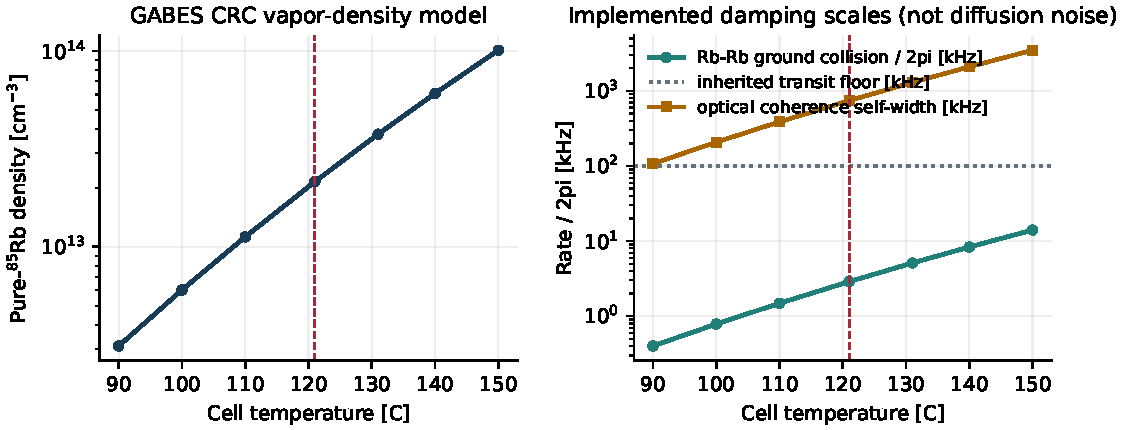
\includegraphics[width=\textwidth]{vapor_scaling.pdf}
\caption{현재 GABES pure-$^{85}$Rb vapor 모델과 dissipator의 온도 의존성.
오른쪽은 코드에 가정된 계수로 얻은 평균방정식의 감쇠 스케일이며, 계수 불확도와 대응
Langevin diffusion을 유도하지 않았으므로 검증된 rate 또는 noise PSD가 아니다.}
\label{fig:vapor-scaling}
\end{figure}

\begin{table}[H]
\centering
\caption{GABES의 현재 가정으로 재계산한 대표 온도별 값. Optical self-width는
$[\Gamma_{\rm eff}-\Gamma]/2$가 optical coherence에 추가되는 HWHM이며, 표의 유효
숫자는 수치 재현성을 표시할 뿐 물리 계수의 불확도를 뜻하지 않는다.}
\label{tab:vapor-numbers}
\small
\begin{tabular}{C{1.7cm}C{3.0cm}C{2.8cm}C{3.2cm}C{3.0cm}}
\toprule
$T$ & $N$ [m$^{-3}$] & ground collision$/2\pi$ & optical self-width$/2\pi$ &
one-photon Doppler FWHM\\
\midrule
$90\degC$  & $3.11\times10^{18}$ & $0.400\kHz$ & $0.107\MHz$ & $558\MHz$\\
$110\degC$ & $1.12\times10^{19}$ & $1.484\kHz$ & $0.387\MHz$ & $574\MHz$\\
$121\degC$ & $2.15\times10^{19}$ & $2.882\kHz$ & $0.742\MHz$ & $582\MHz$\\
$131\degC$ & $3.76\times10^{19}$ & $5.103\kHz$ & $1.297\MHz$ & $589\MHz$\\
$150\degC$ & $1.01\times10^{20}$ & $14.019\kHz$ & $3.482\MHz$ & $603\MHz$\\
\bottomrule
\end{tabular}
\end{table}

$121\degC$에서 GABES가 별도로 입력하는 transit/residual floor는 $100\kHz$이므로,
현재 binary Rb--Rb ground-dephasing 추정 $2.882\kHz$보다 크다. $330\,\mu\mathrm m$와
$530\,\mu\mathrm m$ waist에 대해 2차원 thermal mean speed로 얻은 단순 transit
$1/(2\pi\tau)$는 각각 $119\kHz$, $74\kHz$로 이 floor와 같은 자릿수다. 반면
optical self-broadening은 $0.742\MHz$ HWHM으로 훨씬 크다. 이 비교는 어느 항이
noise power를 지배하는지 말하지 않는다. $D(\Omega)$가 population과 collapse
channel에 따라 다르기 때문이다. 특히 ground collision cross section
$1.9\times10^{-18}\,\mathrm{m^2}$와 self-broadening coefficient
$\beta/2\pi=0.69\times10^{-7}\,\mathrm{Hz\,cm^3}$는 현재 코드에 내장된 가정이며,
원자료 불확도나 apparatus별 보정을 이 계산에서 전파하지 않았다.

\subsection{SABES EOM/etalon power ledger}

\begin{figure}[H]
\centering
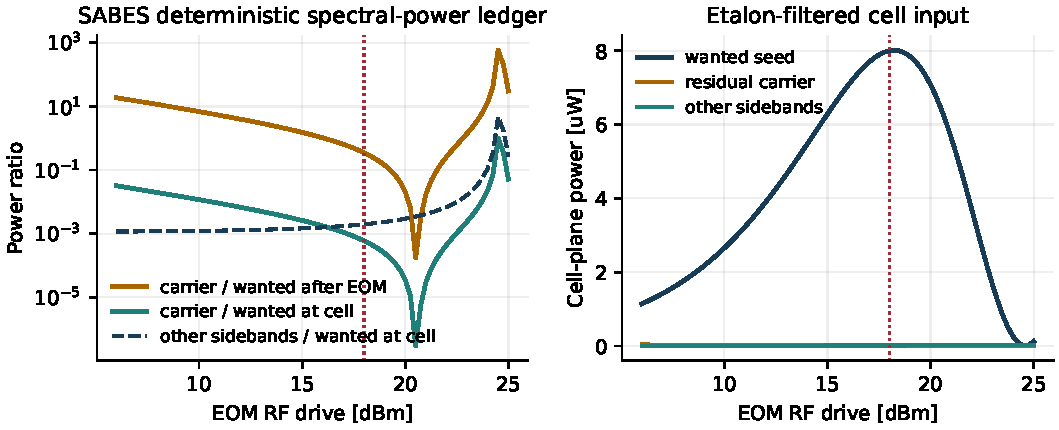
\includegraphics[width=\textwidth]{eom_chain.pdf}
\caption{현재 SABES calibration에서 EOM RF drive를 바꾼 deterministic power sweep.
Bessel sideband power와 etalon transmission만 포함하며 laser/RF phase noise와
원자 매질 전달은 포함하지 않는다.}
\label{fig:eom-chain}
\end{figure}

기본 $18\,\mathrm{dBm}$에서 EOM 직후 residual carrier/wanted-sideband power ratio는
$0.3496$이고, 3단 etalon과 delivery optics 뒤 cell plane에서는
$5.963\times10^{-4}=0.0596\%$이다. 원하는 seed는 $8.000\,\mu\mathrm W$,
other-sideband/wanted ratio는 $0.1968\%$, 계산된 spectral purity는 $99.744\%$이다.
이는 Sim의 cleanest condition과 정성적으로 맞지만, calibration 기반 모델값이지
independent spectrum measurement가 아니다. 특히 이 ledger가 $F_U=1$인지, ECDL/EOM
technical noise가 얼마인지, unwanted mode가 cell에서 어떤 gain을 받는지는 계산하지
않는다.

\subsection{2차원 Maxwell-averaged analysis-frequency response}

\begin{figure}[H]
\centering
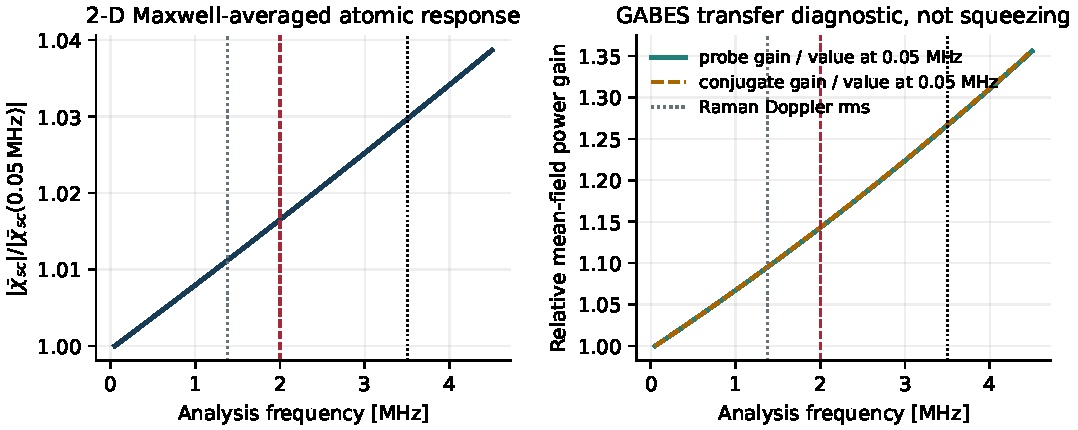
\includegraphics[width=\textwidth]{frequency_response.pdf}
\caption{$T=121\degC$, $\Delta/2\pi=0.9\GHz$,
$\delta/2\pi=-8\MHz$, pump $600\,\mathrm{mW}$, crossing angle $0.32^\circ$에서
GABES pump-only weak response를 $32\times32$ velocity quadrature로 계산한 결과.
세로선은 $1.380\MHz$ Raman Doppler rms, 현 setup에서 반복된 feature의 대표
중심주파수 $2.0\MHz$, 약 $3.5\MHz$ squeezing edge를 표시한다. 실제 feature는
시기와 조건에 따라 대략 $1.5$--$2.4\MHz$에 걸친다. 곡선은 결정론적
susceptibility/gain이고 noise spectrum이 아니다.}
\label{fig:frequency-response}
\end{figure}

분석주파수 $0.05$--$4.5\MHz$에서 $|\bar\chi_{sc}|$는 기준값 대비 약 $3.87\%$
증가하고 mean-field probe gain은 $405.7$에서 $550.1$로 변한다. 절대 gain은 현재
reduced model이 실험 gain을 크게 과대평가한다는 기존 감사 결과 때문에 정량 예측으로
쓰지 않는다. 이 deterministic 계산은 대표 $2\MHz$에 별도 peak를 만들지 않고,
measured $3.5\MHz$ squeezing edge도 정의하지 않는다. 따라서 현 setup의 feature를
GABES atomic pole 또는 Palmer의 servo resonance와 수치적으로 같다고 선언할 근거가
없다.

$18$, $24$, $32$ order/axis를 비교했을 때 complex $\chi_{sc}$의 $18$ 대 $32$ 최대
차이는 $32$-order peak의 $2.14\times10^{-10}$, $24$ 대 $32$는
$1.12\times10^{-13}$이었다. 따라서 이 operating point와 cutoff에서 그림의
quadrature 오차는 표시 정밀도보다 충분히 작지만, 이는 reduced atomic model 자체의
타당성이나 squeezing 예측을 검증하지 않는다.

Quadrature Raman Doppler rms는 $1.38016\MHz$, analytic budget은
$1.38017\MHz$로 일치한다. 이 Gaussian rms를 Lorentzian collision HWHM과 단순히
제곱합하여 squeezing bandwidth라고 부를 수 없다. 최종 bandwidth는 각 velocity
class의 complex response, diffusion, group delay와 detector transfer가 합쳐진
$S_-(\Omega)$에서 읽어야 한다.

%======================================================================
\section{Sim의 plotted-SQL-above carrier trace에 대한 가능한 해석}
%======================================================================

식~\eqref{eq:coherent-bound}를 받아들이면 가능한 해석은 논리적으로 제한된다.
\begin{enumerate}
\item \textbf{Carrier가 cell을 통과하며 더 이상 단순 coherent spectator가 아니다.}
Residual carrier가 pump/desired seed와 추가 Raman/FWM 또는 two-beam-coupling channel을
만들고, vacuum/atomic noise를 증폭하거나 desired twin-beam covariance를 바꾼다.
\item \textbf{Carrier는 coherent이지만 그 amplitude/phase가 classical하게 흔들린다.}
ECDL frequency noise, TA RIN 또는 EOM RF AM/PM noise가 원자 dispersion을 통해
one-sided amplitude noise로 변환된다.
\item \textbf{차동 검출이 그 mode에 대해 balanced가 아니다.}
원하는 probe/conjugate는 balance되어도 residual carrier는 한 arm에만 있거나
$H_p/H_c$, delay, detector saturation이 달라 common noise가 남는다.
\item \textbf{SQL reference가 같은 optical/electronic mode를 갖지 않는다.}
Cell 앞 pump split으로 얻은 SQL과 FWM output의 spectrum, responsivity, detector loading,
RBW/VBW 또는 dark subtraction이 다르면 0-dB 선이 같은 분모가 아니다.
\item \textbf{Beat/intermodulation이 분석 대역으로 내려온다.}
EOM line spacing 자체는 GHz이므로 선형 검출에서 자동으로 내려오지 않는다. 다만
atom-mediated PM-to-AM 변환, detector/TIA 비선형, RF pickup, mixer 또는 aliasing이
명시적으로 있으면 MHz feature를 만들 수 있다.
\end{enumerate}

내부 랩미팅 자료와 실험 로그는 near-$2\MHz$ feature의 반복성을 확립하지만 하나의
전달 경로를 고르지는 못한다. 논문과 내부 기록에는 residual carrier의 cell-bypass
RIN, pump-off hot-cell trace, post-cell carrier filtering, etalon slope, 주파수별
CMRR/transfer를 같은 조건에서 묶은 측정이 없다. 따라서 pure coherent admixture
모형만으로 plotted-SQL-above carrier trace를 설명할 수 없다는 결론은 유지된다.
반면 near-$2\MHz$ feature를 ECDL 고유 공명, collision/thermal noise 또는 broadband
excess-noise floor와 동일시하는 것은 \openclaim 이다.

%======================================================================
\section{가장 판별력이 큰 후속 실험}
%======================================================================

\subsection{우선순위 1: 원자 밖에서 coherent-bound 검증}

\begin{enumerate}
\item Cell을 완전히 우회하고, 실제 EOM/etalon chain으로 carrier/wanted ratio를
$\ll0.5\%$부터 $50\%$까지 바꾼다.
\item 두 detector의 총 power와 전자 gain을 실제 FWM 측정과 같게 맞춘다.
\item 각 ratio에서 total detected power로 SQL slope를 다시 측정한다.
\end{enumerate}
이 상태에서 ratio가 커질수록 SQL 위로 가면 원자 매질이 아니라 EOM/laser/detector
technical path가 이미 충분하다. 모든 ratio가 SQL이면 원자-mediated transfer가
필요하다는 강한 증거가 된다.

\subsection{우선순위 2: 단계별 on/off matrix}

동일한 acquisition 설정으로 다음 순서를 비교한다.
\begin{equation*}
\text{laser only}\rightarrow
\text{cold cell}\rightarrow
\text{hot cell, pump off}\rightarrow
\text{pump on, phase mismatch}\rightarrow
\text{optimal FWM}.
\end{equation*}
각 단계에서 single-arm RIN, cross spectrum $S_{pc}$, difference PSD, 총 power SQL을
함께 저장한다. Hot-cell/pump-off에서 생기면 absorption/phase-to-amplitude conversion,
pump-on/mismatched에서 생기면 pump scatter 또는 parasitic nonlinear channel,
optimal condition에서만 생기면 desired gain/covariance와 연결된 기작이다.

\subsection{우선순위 3: carrier가 noise를 어디에서 전달하는지 찾기}

\begin{itemize}
\item \textbf{Post-cell narrow filtering:} cell 뒤에서 residual carrier만 제거한다.
Noise가 함께 사라지면 detector direct admixture가 유력하고, carrier를 제거해도 desired
probe/conjugate noise가 남으면 cell 내부에서 이미 잡음이 전달된 것이다.
\item \textbf{Relative phase/angle/overlap:} pure Poisson admixture는 optical phase에
무관하지만 atomic grating/two-beam coupling은 phase, crossing angle, imaging plane,
seed power에 민감하다.
\item \textbf{Side fluorescence:} $90^\circ$ fluorescence spectrum과 forward noise를
동시 측정하여 isotropic Raman/fluorescence와 directional phase-matched FWM을 구분한다.
\end{itemize}

\subsection{우선순위 4: 1.8--2 MHz feature의 전달 경로 분리}

Peak 높이 하나만 비교하지 말고 (i) narrow peak의 중심ㆍ적분 power, (ii) 인접
off-peak pedestal, (iii) $40$--$500\kHz$ squeezing, (iv) 동일조건 SQL을 각 switch
상태에서 함께 기록한다. 사용하지 않는 laser/driver/RF supply를 전원선까지 분리하고,
PZT/MOPA 전원, passive filter, noise eater를 하나씩 on/off한다. EOM drive와 seed/FWM
gain을 고정한 채 etalon 1ㆍ2ㆍ3개 및 bypass를 비교하고, PZT scan으로 peak와
$dT/d\nu$의 상관을 측정한다. 이어 EOM frequency를 scan하여 peak가 FWM gain slope
$dG/d\nu$와 함께 변하는지 확인한다\cite{ExperimentLog20260713}.

Servo gain, actuator, filter corner, lock point를 바꾸면서 중심주파수도 추적한다.
Unity-gain/servo resonance와 함께 움직이면 laser electronics가 유력하고, temperature,
one/two-photon detuning, pump power, crossing angle과 함께 움직이면 atomic conversion이
유력하다. Fast photodiode RIN과 frequency discriminator로 laser amplitude 및
frequency-noise PSD를 측정하고, 식~\eqref{eq:gain-sensitivity}의 measured derivative로
difference-noise 크기를 예측한다. Narrow peak, 완만한 high-frequency roll-off와
carrier-dependent broadband degradation은 세 개의 독립 진단축으로 유지한다.

\subsection{우선순위 5: detector transfer와 saturation}

동일한 shot-noise-limited beam을 50:50으로 나누어
$H_p(\Omega),H_c(\Omega)$, CMRR, differential delay, cross talk를
$0.05$--$5\MHz$에서 측정한다. Optical power를 넓게 sweep해 shot noise의 선형성,
TIA compression, photodiode saturation, intermodulation을 확인한다. DC balance 한
점만으로 RF balance를 증명할 수 없다.

\subsection{우선순위 6: atomic thermal mechanism 분리}

\begin{itemize}
\item Waist를 바꿔 noise corner가 $v_\perp/w$로 움직이는지 본다.
\item Temperature와 cell length를 독립적으로 바꿔 density, integrated OD, transit을
분리한다.
\item Buffer gas 또는 wall coating이 다른 cell을 사용해 collision/transit을 바꾼다.
\item Pump-off decay와 fluorescence tail의 density/geometry scaling으로 radiation
trapping을 확인한다.
\item Magnetic field와 polarization을 바꿔 spin/population-noise coupling을 검사한다.
\end{itemize}

%======================================================================
\section{결론과 claim ledger}
%======================================================================

\begin{table}[H]
\centering
\caption{본 조사에서 허용되는 최종 claim과 아직 열린 claim.}
\label{tab:claim-ledger}
\small
\begin{tabularx}{\textwidth}{L{2.5cm}Y}
\toprule
상태 & 판정\\
\midrule
\established & 동일조건 SQL로 정규화한 독립 coherent admixture와 대칭ㆍ공분산 정합
post-loss는 $R\le1$을 유지한다. 비대칭 loss에는 일반화할 수 없다.\\
\established & Sim 논문은 정확히 $50\%$ residual-carrier spectrum이 논문에 그려진
SQL reference 위에 나타남을 보이지만 $50\%$ slope scaling은 제시하지 않는다.\\
\established & Sim Fig.~3(a)의 같은 spectrum에서 $40$--$500\kHz$의 직접
$-7.8\dB$ IDS와 near-$2\MHz$ peak가 공존한다. 내부 자료는 대략
$1.5$--$2.4\MHz$ feature의 반복을 보인다.\\
\inferred & 이 feature는 해당 주파수의 squeezing과 usable bandwidth를 국소적으로
훼손하지만, 저주파ㆍbroadband excess-noise floor의 주원인일 필요는 없다.\\
\openclaim & Sim의 입력비와 post-cell detected shot-weight 비가 같지 않으므로
$C_{\rm proxy}\simeq4.26$은 Fano factor나 excess-noise transfer로 식별되지 않는다.\\
GABES 계산 & 현재 코드 가정에서 $121\degC$의 $N=2.15\times10^{19}\,\mathrm{m}^{-3}$,
ground collision $2.882\kHz$, optical self-width $0.742\MHz$, non-collinear
Raman Doppler rms $1.380\MHz$이다. 이들은 noise PSD가 아니다.\\
GABES 계산 & SABES 기본 $18\,\mathrm{dBm}$ power ledger의 cell-plane carrier/wanted
ratio는 $0.0596\%$이나, 이는 independent spectrum/noise 측정이 아니다.\\
\openclaim & Sim의 plotted-SQL-above trace가 엄밀한 동일조건 SQL도 넘는지, 그리고
laser electronics, atom-mediated parasitic
mixing, collision/fluorescence, detector mismatch 또는 SQL calibration 중 무엇에
주로 기인하는지는 현재 데이터로 결정되지 않는다.\\
\openclaim & 반복되는 near-$2\MHz$ feature의 주 전달 경로가 laser/PZT/MOPA 전원,
RF driver, etalon $dT/d\nu$, FWM $dG/d\nu$, PD RF imbalance 또는 filter self-resonance
중 무엇인지는 분리되지 않았다.\\
\openclaim & 현재 GABES는 microscopic $D(\Omega)$와 detector transfer가 없어
physical squeezing magnitude와 bandwidth를 예측하지 않는다.\\
\bottomrule
\end{tabularx}
\end{table}

최종적으로 사용자의 직관은 조건부로 옳다. 펌프에서 유래한 이상적인 EOM
sideband라면 coherent이고 Poissonian이므로 단순 혼입만으로 SQL을 넘지 않는다.
바로 그 정리 때문에 Sim의 $50\%$ plotted-SQL-above trace는 더 흥미로운 진단이 된다.
실제 sideband는 noisy RF/ECDL에서 생성되고, 뜨거운 비선형 원자 매질과 서로 다른
mode transfer를 거치며, finite-CMRR detector에 한쪽으로 들어간다. 이 전체 channel의
출력은 더 이상 독립 coherent spectator일 필요가 없다. 다음 단계는 carrier를
제거하는 데 그치지 않고, 위 on/off matrix와 covariance-calibrated measurement로
어느 단계에서 $F_U>1$ 또는 $S_{pc}$ 손실이 생기는지를 찾는 것이다.

Near-$2\MHz$ feature는 이 carrier-dependent broadband degradation과 분리해야 한다.
동일한 Sim spectrum에서 저주파 $-7.8\dB$가 유지되므로 narrow peak가 최적 squeezing
depth를 정하지는 않는다. 그러나 여러 내부 자료에서 반복되고 일부 trace에서는 해당
대역의 squeezing을 지우거나 plotted SQL 위로 올리므로, usable bandwidth를 확보하려면
독립적인 전원ㆍlaserㆍetalonㆍFWMㆍdetector transfer audit가 필요하다.

%======================================================================
\appendix
\section{수치 재현과 산출물}
%======================================================================

모든 그림과 표의 계산은 \path{scripts/generate_analysis.py}에서 재현된다. 저장소
root에서 다음 명령을 실행한다.
\begin{verbatim}
python docs\fwm_thermal_excess_noise_report\scripts\generate_analysis.py
\end{verbatim}
산출물은 다음과 같다.
\begin{itemize}
\item \path{data/analysis_summary.json}: 모든 입력, claim gate, 진단값, runtime 및
분석 스크립트 및 로컬 GABES/SABES Python source snapshot의 SHA-256;
\item \path{data/noise_mixing.csv}: $r,F$ sweep과 SQL crossing threshold;
\item \path{data/vapor_scaling.csv}: density, collision, self-width, Doppler scale;
\item \path{data/eom_sweep.csv}: EOM 전후 및 cell-plane sideband power;
\item \path{data/frequency_response.csv}: 2D Maxwell-averaged $\bar\chi$와 mean-field gain;
\item \path{figures/*.pdf}: 본문에 포함된 네 개의 vector figure.
\end{itemize}

실행 당시 Git HEAD는
\texttt{c964a724b1ad370e53af1a89c78f8df04fd37983}이며 tracked worktree가 이미 dirty였다.
스크립트는 output write 전에 상태를 snapshot하고 현재 worktree 코드를 직접
import하므로, commit만으로 입력을 복원할 수 없다. JSON에 Git 상태, Python/NumPy/
Matplotlib 버전과 분석 스크립트 및 로컬 GABES/SABES 패키지의 모든
\texttt{.py} 파일 SHA-256을 함께 저장했다. 이는 현재 import closure의 보수적
superset이므로 간접 의존성과 dirty source도 기록한다. 본 보고서
생성은 기존 코드나 문서를 수정하지 않고 새 폴더 안에만 파일을 추가했다.

\section{Coherent-bound의 multimode 확장}

Detector $p$에 들어오는 독립 coherent mode를 $N_{p,m}$, detector $c$의 mode를
$N_{c,n}$라 하자. 각 mode가 Poisson이고 mutual beat가 acquisition band 밖이면
\begin{equation}
N_p=\sum_mN_{p,m}\sim\operatorname{Pois}\!\left(\sum_m\mu_{p,m}\right),
\quad
N_c=\sum_nN_{c,n}\sim\operatorname{Pois}\!\left(\sum_n\mu_{c,n}\right).
\end{equation}
그러므로
\begin{equation}
\Var(N_p-wN_c)=\sum_m\mu_{p,m}+w^2\sum_n\mu_{c,n},
\end{equation}
이고 이는 모든 detected coherent power를 포함한 동일조건 SQL과 같다. Spatial,
polarization, frequency label은 이 결론을 바꾸지 않는다. 결론을 바꾸는 것은
(i) $F_m\ne1$, (ii) mode 사이 classical correlation/anticorrelation,
(iii) beat가 검출 대역에 들어옴, (iv) detector의 비선형성, 또는
(v) SQL 분모가 같은 mode/transfer를 갖지 않는 경우다.

\section{권장 GABES 구현 순서}

물리적 squeezing 계산을 추가할 때의 최소 순서는 다음과 같다.
\begin{enumerate}
\item Pumped steady state의 각 velocity class에 대해 full Zeeman/polarization Jacobian
$A_{\bm v}$와 field-coupling matrix를 구성한다.
\item 모든 collapse channel에서 operator diffusion을 generalized Einstein relation으로
유도하고 steady-state population dependence를 보존한다.
\item Atomic variables를 제거해 $M_q(\Omega),B(\Omega),D(\Omega)$를 만들고
식~\eqref{eq:physical-realizability}을 검증한다.
\item Collisionless/fixed-velocity 근사에서는 class별 covariance를 합한다. Velocity-
changing collision을 켜면 class 간 drift/diffusion을 포함한 joint covariance를 만들고,
longitudinal segment마다 Van Loan block exponential로 식~\eqref{eq:lyapunov}를 적분한다.
\item Wanted seed, residual carrier, other EOM sidebands 및 생성된 conjugates를 하나의
multimode Gaussian vector로 확장한다. 각 mode의 spatial overlap과 phase를 보존한다.
\item Cell 뒤 loss와 measured $H_p,H_c,w,S_{\rm el}$를 적용하고 동일조건 SQL로
식~\eqref{eq:final-observable}을 정규화한다.
\item No-coupling, passive loss, ideal $SU(1,1)$, zero length,
commutator preservation, positive-semidefinite covariance의 limiting tests를 고정한다.
\item Sim의 clean-carrier point를 calibration에 사용했다면 다른 carrier ratio, 온도,
detuning, analysis frequency를 held-out validation으로 남긴다.
\end{enumerate}
이 구현 전에는 GABES의 mean-field gain이나 commutator-completion vacuum fixture를
atomic Langevin corrected squeezing으로 이름 붙이지 않는 것이 중요하다.

\clearpage
\renewcommand{\refname}{참고문헌}
\bibliographystyle{unsrt}
\bibliography{references}

\end{document}
